%这个是根据计算机学报官网下的LaTeX模板改的,主要修改内容:①把GBK编码改成了UTF-8编码。②引入zhwinfonts,用上传的字体文件实现了字体的使用。
%现存的问题:①中文无法使用加粗功能,但是英文可以。解决方式1:使用黑体来凑合代替。解决方式2:在PDF编辑器里面一个一个加粗。②无法实现模板中所要求的每页脚注从1开始的要求。
%如果您在使用该模板的过程中遇到问题,或者有对该模板的修改意见,请联系本人:微信PolarisRisingWar(诸神缄默不语),或者CSDN诸神缄默不语(PolarisRisingWar)

\documentclass[10.5pt,compsoc,twocolumn]{CjC}

%% ------------------- 导言区 ------------------- %%
\usepackage{caption}

%% ------------------------ 该文件为导言文件 ------------------------

% \usepackage{ctex}
% \setCJKmainfont{仿宋}

% 使用fancyhdr包设置不同页面的不同页眉页脚。
\usepackage{fancyhdr}


\usepackage{svg}
\usepackage{CJKutf8}
%\usepackage{CJK}
\usepackage{graphicx}
\usepackage{footmisc}
\usepackage{subfigure}
\usepackage{url}
\usepackage{multirow}
\usepackage[noadjust]{cite}
\usepackage{amsmath,amsthm}
\usepackage{amssymb,amsfonts}
\usepackage{booktabs}
\usepackage{color}
\usepackage{ccaption}
\usepackage{booktabs}
\usepackage{float}
\usepackage{fancyhdr}
\usepackage{caption}
\usepackage{xcolor,stfloats}
\usepackage{comment}
\setcounter{page}{1}
\graphicspath{{figures/}}
\usepackage{cuted}%flushend,
\usepackage{captionhack}
\usepackage{epstopdf}
\usepackage[utf8]{inputenc}

\usepackage{cite}
\usepackage[hidelinks]{hyperref} %使引用文献可以跳转的包
\usepackage{booktabs} % 画三线表的包
\usepackage{array}
%\usepackage{ccmap}
%\CJKtilde
%\usepackage{CJKpunct} 
%\usepackage[lite,subscriptcorrection,slantedGreek,nofontinfo]{mtpro2}

%===============================%

%\firstfootname{ \quad \quad }
\headevenname{\mbox{\quad} \hfill  \mbox{\zihao{-5}{\begin{CJK*}{UTF8}{song}数字建模与智能决策赛道\end{CJK*}} \hspace {50mm} \mbox{\begin{CJK*}{UTF8}{song}2024 年\end{CJK*}}}}%
\headoddname{\begin{CJK*}{UTF8}{song}第二届 \hfill 全国仿真创新应用大赛\end{CJK*}}%

%footnote use of *
\renewcommand{\thefootnote}{\fnsymbol{footnote}}
\setcounter{footnote}{0}
\renewcommand\footnotelayout{\zihao{5-}}

\newtheoremstyle{mystyle}{0pt}{0pt}{\normalfont}{1em}{\bf}{}{1em}{}
\theoremstyle{mystyle}
\renewcommand\figurename{figure~}
\renewcommand{\thesubfigure}{(\alph{subfigure})}
\newcommand{\upcite}[1]{\textsuperscript{\cite{#1}}}
\renewcommand{\labelenumi}{(\arabic{enumi})}
\newcommand{\tabincell}[2]{\begin{tabular}{@{}#1@{}}#2\end{tabular}}
\newcommand{\abc}{\color{white}\vrule width 2pt}
\makeatletter
\renewcommand{\@biblabel}[1]{[#1]\hfill}
\makeatother
\setlength\parindent{2em}
%\renewcommand{\hth}{\begin{CJK*}{UTF8}{zhhei}}
%\renewcommand{\htss}{\begin{CJK*}{UTF8}{song}}
\bibliographystyle{IEEEtran} % 这里的 IEEEtran 文件的后缀为 .bst
\input{zhwinfonts}
\def\vspaceLen{2mm}

% 定义首页页眉页脚
\fancypagestyle{firstpage}{
    \fancyhf{} %清空页眉页脚
    \fancyhead[L]{
        % 定义页眉
            \zihao{5-}\begin{CJK*}{UTF8}{song}第??卷\quad 第?期 \end{CJK*}\\
            \vspace{\vspaceLen}
            \zihao{5-}\begin{CJK*}{UTF8}{song}20??年?月 \end{CJK*}
    }

    \fancyhead[C]{
        % 定义页眉
            \zihao{5-}\begin{CJK*}{UTF8}{song}计\quad 算\quad 机\quad 学\quad 报\end{CJK*}\\
            \vspace{\vspaceLen}
            \zihao{5-}\begin{CJK*}{UTF8}{song}CHINESE JOURNAL OF COMPUTERS \end{CJK*}
    }

    \fancyhead[R]{
        % 定义页眉
            \zihao{5-}\begin{CJK*}{UTF8}{song}Vol. ??  No. ?\end{CJK*}\\
            \vspace{\vspaceLen}
            \zihao{5-}\begin{CJK*}{UTF8}{song}???. 20??\end{CJK*}
    }
    \fancyfoot[L]{
        \begin{tabular}{p{0.05cm}p{16.15cm}}
            \multicolumn{2}{l}{\rule[4mm]{40mm}{0.1mm}}\\[-3mm]
            &
            \begin{CJK*}{UTF8}{song}
              此处填写页脚
            \end{CJK*}
        \end{tabular}
    }
}


% 定义双数页页眉页脚
\fancypagestyle{evenpages}{
    \fancyhf{} %清空页眉页脚
    \fancyhead[L]{
        % 定义页眉
            \zihao{5-}\begin{CJK*}{UTF8}{song}第??卷\quad 第?期 \end{CJK*}\\
            \vspace{\vspaceLen}
            \zihao{5-}\begin{CJK*}{UTF8}{song}20??年?月 \end{CJK*}
    }

    \fancyhead[C]{
        % 定义页眉
            \zihao{5-}\begin{CJK*}{UTF8}{song}计\quad 算\quad 机\quad 学\quad 报\end{CJK*}\\
            \vspace{\vspaceLen}
            \zihao{5-}\begin{CJK*}{UTF8}{song}CHINESE JOURNAL OF COMPUTERS \end{CJK*}
    }

    \fancyhead[R]{
        % 定义页眉
            \zihao{5-}\begin{CJK*}{UTF8}{song}Vol. ??  No. ?\end{CJK*}\\
            \vspace{\vspaceLen}
            \zihao{5-}\begin{CJK*}{UTF8}{song}???. 20??\end{CJK*}
    }
    \fancyfoot[L]{
        \begin{tabular}{p{0.05cm}p{16.15cm}}
            \multicolumn{2}{l}{\rule[4mm]{40mm}{0.1mm}}\\[-3mm]
            &
            \begin{CJK*}{UTF8}{song}
              此处填写页脚
            \end{CJK*}
        \end{tabular}
    }
}

% 偶数页页眉页脚设置
\fancyhead[LE]{\zihao{5-}\begin{CJK*}{UTF8}{song}\thepage \end{CJK*}}
\fancyhead[CE]{\zihao{5-}\begin{CJK*}{UTF8}{song}计 \quad 算 \quad 机 \quad 学 \quad 报 \end{CJK*}}
\fancyfoot[RE]{\zihao{5-}\begin{CJK*}{UTF8}{song}2024 年\end{CJK*}}

% 奇数页页眉页脚设置
\fancyhead[LO]{\zihao{5-}\begin{CJK*}{UTF8}{song}? 期 \end{CJK*}}
\fancyhead[CO]{\zihao{5-}\begin{CJK*}{UTF8}{song}作者姓名等:论文题目\end{CJK*}}
\fancyfoot[RO]{\zihao{5-}\begin{CJK*}{UTF8}{song} \thepage \end{CJK*}}




%% ------------------- 正文区 ------------------- %%
\begin{document}
% 引入一些定义
\hyphenpenalty=50000
\makeatletter
\newcommand\mysmall{\@setfontsize\mysmall{7}{9.5}}
\newenvironment{tablehere}
  {\def\@captype{table}}

\let\temp\footnote
\renewcommand \footnote[1]{\temp{\zihao{-5}#1}}


\thispagestyle{plain}%
\thispagestyle{empty}%
\pagestyle{CjCheadings}

\onecolumn % 该命令表示本页为单栏页面
\thispagestyle{firstpage} %为首页设置页眉。使用preamble/header_def.tex文件中定义的页眉


    
    
    % 定义标题
    \centering
    \vspace {11mm}
    \begin{CJK*}{UTF8}{zhhei}
    {
      \zihao{2} 题目(中英文题目一致)字体为2号黑体(全文除特别声明外, 外文统一用Times New Roman) 
    }
    \end{CJK*}
    
    \vskip 5mm
    
    % 定义作者
    {
      \zihao{3}
      \begin{CJK*}{UTF8}{fs}
        作者名$^{1)}$\quad  作者名$^{2),3)}$ \quad 作者名$^{3) }$($^*$字体为3号仿宋*作者)
      \end{CJK*}
    }
    
    \vspace {5mm}
    
    % 定义中文作者单位1
    \zihao{6}{\begin{CJK*}{UTF8}{song}
    $^{1)}$(单位全名 部门(系)全名, 市(或直辖市) 国家名 邮政编码)
    *字体为6号宋体*单位
    \end{CJK*}}
    
    % 定义中文作者单位2
    \zihao{6}{\begin{CJK*}{UTF8}{song}
    $^{2)}$(单位全名 部门(系)全名, 市(或直辖市) 国家名
    邮政编码)*中英文单位名称、作者姓名须一致*
    \end{CJK*}}
    
    % 定义中文作者单位3
    \zihao{6}{\begin{CJK*}{UTF8}{song}
    $^{3)}$(单位全名 部门(系)全名, 市(或直辖市) 国家名 邮政编码)
    \end{CJK*}}
    
    % 定义中文作者单位4
    \zihao{6}{\begin{CJK*}{UTF8}{zhhei}
    论文定稿后,作者署名、单位无特殊情况不能变更。若变更,须提交签章申请,国家名为中国可以不写,省会城市不写省的名称,其他国家必须写国家名。
    \end{CJK*}}
    
    % \vskip 命令在 LaTeX 中用于在垂直方向上插入可调节的空间。它可以在文档中增加或减少行间距、段落间距,或在图形、表格和文本之间插入额外的空白。
    \vskip 5mm
    
    {
      \centering
      \begin{tabular}{p{160mm}}
        % 定义中文摘要
        \zihao{5-}{
          \setlength{\baselineskip}{16pt}
          \selectfont{
            \noindent\begin{CJK*}{UTF8}{zhhei}摘\quad 要\quad \end{CJK*} 
            \begin{CJK*}{UTF8}{song}
              *中文摘要内容置于此处(英文摘要中要有这些内容),字体为小5号宋体。摘要贡献部分,要有数据支持,不要出现``...大大提高''、``...显著改善''等描述,正确的描述是``比{\ldots}提高X{\%}''、
              ``在{\ldots}上改善X{\%}''。*摘要
            \end{CJK*}\par
          }
        }\\[2mm]
        
        % 定义中文关键词
        \zihao{5-}{
          \noindent
          \begin{CJK*}{UTF8}{zhhei}
            关键词\end{CJK*} \quad \begin{CJK*}{UTF8}{song}{*关键词(中文关键字与英文关键字对应且一致,应有5-7个关键词);关键词;关键词;关键词*  }
          \end{CJK*}
        }\\[2mm]
    
        % 定义中图法分类号、TP、DOI号
        \zihao{5-}{
          \begin{CJK*}{UTF8}{zhhei} 中图法分类号 \end{CJK*}	
          \begin{CJK*}{UTF8}{song} TP \end{CJK*}
          \rm{\quad \quad \quad}
          \begin{CJK*}{UTF8}{zhhei} DOI号: \end{CJK*}
          \begin{CJK*}{UTF8}{song}
        *投稿时不提供DOI号\end{CJK*}
        }
      \end{tabular}
    }
    
    \vskip 7mm
    
    % 英文标题
    \begin{center}
      \zihao{3}{
        {
          \begin{CJK*}{UTF8}{zhhei}
            Title *(中英文题目一致)字体为4号Times New Roman,加粗* Title
          \end{CJK*}
        }
      }\\
    
      % 英文作者
      \vspace {5mm}
      \zihao{5}{ {
        \begin{CJK*}{UTF8}{zhhei}
          NAME Name-Name$^{1)}$ NAME Name$^{2)}$ NAME Name-Name$^{3)}$ *字体为5号Times new Roman*Name
        \end{CJK*}
      }}\\
    
      \vspace {2mm}
      % 英文作者单位1
      \zihao{6}{
        \begin{CJK*}{UTF8}{zhhei}{$^{1)}$(Department of ****, University, City ZipCode, China) *字体为6号Times new Roman* Depart.Correspond}\end{CJK*}
      }
    
      % 英文作者单位2
      \zihao{6}{
        \begin{CJK*}{UTF8}{zhhei}{$^{2)}$(Department of ****, University, City ZipCode)*中国不写国家名*}\end{CJK*}
      }
    
      % 英文作者单位3
      \zihao{6}{
        \begin{CJK*}{UTF8}{zhhei}{$^{3)}$(Department of ****, University, City ZipCode, country)*外国写国家名*}\end{CJK*}
        }
    
    \end{center}
    
    
    \begin{tabular}{p{160mm}}
      % 英文摘要标题:Abstract
      \zihao{5}{
        \setlength{\baselineskip}{18pt}
        \selectfont{
          {\bf Abstract}\quad
          \begin{CJK*}{UTF8}{zhhei}(\textbf{500英文单词,内容包含中文摘要的内容}).字体为Times new Roman,字号5号* Abstract\end{CJK*}
          \par
        }
      }\\
    
      % 英文摘要内容
      \setlength{\baselineskip}{18pt}
      \selectfont{
        \zihao{5}{
          \noindent Do not modify the amount of space before and after the artworks. One- or two-column format artworks are preferred. and Tables, create a new break line and paste the resized artworks where desired. Do not modify the amount of space before and after the artworks. One- or two-column format artworks are preferred. All Schemes, Equations, Figures, and Tables should be mentioned in the text consecutively and numbered with Arabic numerals, and appear below where they are mentioned for the first time in the main text. To insert Schemes, Equations, Figures, and Tables, create a new break line and paste the resized artworks where desired. Do not modify the amount of space before and after the artworks. One- or two-column format artworks are preferred.Do not modify the amount of space before and after the artworks. One- or two-column format artworks are preferred. and Tables, create a new break line and paste the resized artworks where desired. Do not modify the amount of space before and after the artworks. One- or two-column format artworks are preferred. All Schemes, Equations, Figures, and Tables should be mentioned in the text consecutively and numbered with Arabic numerals, and appear below where they are mentioned for the first time in the main text.
    
          \vspace {5mm}
    
          % 英文关键词
          {\bf Keywords}\quad
          \begin{CJK*}{UTF8}{zhhei}
            中文关键字与英文关键字对应且一致,\textbf{不要用英文缩写}); key word; key word; key word* *字体为5号Times new Roman * Key words
          \end{CJK*}
        }
        \par
      }
    \end{tabular}
    
    % \setlength{\tabcolsep}{2pt}



\clearpage \clearpage % 引入中英文标题、作者、作者单位、关键词

% \begin{strip}
% \vspace {-13mm}
% \end{strip}
%     % \linespread{1.15}

\twocolumn
\begin{CJK*}{UTF8}{fs}
% \input{mainbody/section1.tex}%添加主体
\section{introduction}

A picture is worth a thousand words and excellent artworks frequently provide information distinct from that of real photographs. However, without long-term professional training, an ordinary person may find it difficult to independently create a piece of art that satisfies themselves or others. Moreover, the time and cost required to train a true artist are often immeasurable. Even for a skilled artist proficient in creating stylized works, completing a single art piece requires a amount of time. To efficiently convert real photos into artistic images, the task of image style transfer has emerged.

Image style transfer aims to combine the content of a real photograph with the style of an artwork, creating a stylized image that simultaneously embodies the content of the photograph and the style of the artwork. In style transfer tasks, the image providing the content is referred to as the content image, while the image providing the style is called the style image. The generated result is known as the stylized image. This paper primarily focuses on image style transfer; unless otherwise specified, the term "style transfer" in the following text refers specifically to image style transfer.

The development of style transfer can be divided into two stages. The first stage spans from the mid-1990s\citep{01jing2019neural} to 2016\citep{02gatys2016image}, characterized by the use of mathematical models for texture simulation. The second stage, from 2016\citep{02gatys2016image} to the present, is marked by the use of deep learning and neural networks for style transfer. The former is relatively traditional, while the latter incorporates new methods. Therefore, this paper refers to the first stage as "traditional style transfer" and the second stage as "neural style transfer."

Traditional style transfer typically employs mathematical and signal processing techniques, such as texture synthesis, histogram matching, and filtering. These methods involve manipulating pixels to simulate the desired style. For example, frequency domain filtering can be used to enhance or suppress certain frequency components of an image, thereby altering its appearance. The advantage of traditional style transfer lies in its higher computational speed and lower resource consumption, but it may struggle to capture more advanced artistic styles and textures.

In contrast, neural network-based style transfer methods are more flexible and efficient. Deep learning techniques are used to learn and apply image styles. They train neural networks to capture the features of different artistic styles, which are then applied to the input image to generate a new image with the desired style. The strength of neural style transfer lies in its ability to better capture the details and complexities of artistic styles, though the required time and resource consumption can vary significantly depending on the network structure.

Traditional style transfer and neural style transfer should not be viewed as mutually exclusive. On the contrary, some of the recent neural style transfer advancements\citep{03li2023frequency,04huang2017arbitrary} draw inspiration from traditional style transfer and digital image processing. Meanwhile, neural network-based style transfer techniques also have certain drawbacks, such as artifacts and difficulties in controlling the stylization process. Combining traditional and neural style transfer methods could potentially yield better results.

Image style transfer has a wide range of practical applications, such as in environmental atmosphere rendering\citep{05ke2023neural}, font generation\citep{06fu2023neural}, font recognition\citep{07tang2022few}, portrait editing \citep{08liu2021psgan++,09xu2022transeditor}, design assistance \citep{10liu2021self,11bae2023unsupervised,12hollein2022stylemesh,13yin20213dstylenet,14yang2022industrial}, photo restoration\citep{15gunawan2023modernizing}, virtual reality (VR), and augmented reality (AR)\citep{16mu20223d}.
Furthermore, as a fundamental task in computer vision, style transfer can assist in other research areas, such as adversarial example\citep{17naseer2022stylized,18cao2023stylefool}, image generation\citep{19karras2019style}, and domain adaptation\citep{20guan2022cdtnet}. Whether from the perspective of practical applications or scientific research, the task of style transfer has broad applications.

This paper primarily introduces the task of image style transfer, and its structure is organized as follows. Firstly, it introduces the achievements of traditional style transfer. Secondly, it covers the achievements of the neural style transfer. Thirdly, it presents the evaluation parameters in the style transfer field and compares representative achievements in the field. Fourthly, it discusses the application of style transfer in other fields and non-image style transfer tasks. Finally, it discusses the unresolved issues in the field of style transfer. The main contributions of this paper are as follows:
\begin{enumerate}
    \item Introducing some achievements in style transfer in the chronological order and providing a subdivision method for neural style transfer.
    \item Comparing some representative achievements in the field of style transfer.
    \item Providing a comprehensive summary and analysis of objective evaluation metrics in the field of style transfer. There is considerable debate over the choice of objective metrics in style transfer, with different studies employing a wide variety of metrics that vary significantly. To the best of our knowledge, this is the first work to systematically summarize and analyze the objective evaluation metrics used in the majority of recent style transfer studies.
    \item Discussing the existing issues in the field of style transfer.
\end{enumerate} %添加引言
\begin{CJK*}{UTF8}{zhhei}
    \zihao{5}
    \vskip 1mm
    \section{相关技术}
\end{CJK*}



\begin{CJK*}{UTF8}{zhhei}
    \subsection{图像级弱监督语义分割}
\end{CJK*}

图像级WSSS是所有WSSS方法中挑战性最大的一种。该方法仅依赖于图像的分类标签。与其它形式的弱标注,如涂鸦标注和边框标注相比,图像级标注所提供的信息量更为有限,因此在实现像素级精细分割的任务上难度更高。利用图像级标注的WSSS方法通常生成CAM来获取图像分类时的关注区域,从而捕获特定于类别的定位信息\cite{42ahn2018learning}。但CAM激活的区域通常只会覆盖最明显最具判别力的对象区域,而忽略其它非判别性的区域。一些工作专注于生成高质量CAM,如对抗性擦除方法\cite{04wei2017object},通过擦除最具判别力的对象区域来迫使模型关注其它非判别性的区域,可以一定程度上优化缓解CAM激活不全的问题。还有工作利用子类别探索\cite{05chang2020weakly}、自监督注意力机制\cite{06wang2020self}和多图像语义信息\cite{07li2021group}来获得更精准的CAM。最近也有工作\cite{08xie2022clims,09lin2023clip}利用了CLIP\cite{10radford2021learning}模型,利用CLIP对图像和文本强大的上下文理解能力抑制背景像素的激活,更专注于前景区域。然而这些方法大多集中于多阶段WSSS方法,且需要分阶段地训练模型和不同的训练策略,多个阶段间的复杂交互较为繁琐。本文提出的单阶段WSSS方法SS-EPA,集成了端到端式多头自注意力CAM优化方法,减少了流程复杂性。 

\vspace{2mm}

\begin{figure*}[htbp]
    \centerline{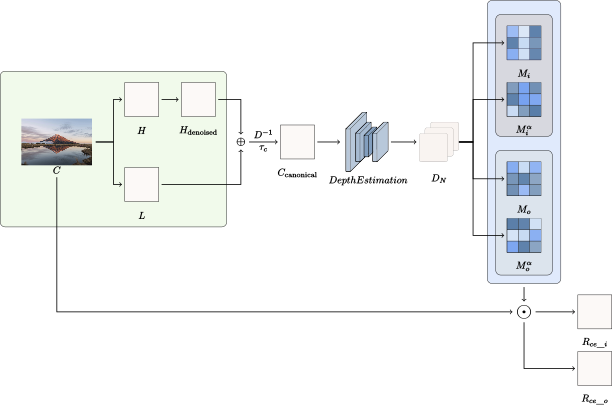
\includegraphics[width=6in]{fig/fig2.pdf}}
    \begin{CJK*}{UTF8}{fs}
        \caption{补丁语义亲和力获取流程图}\label{fig2}
    \end{CJK*}
\end{figure*}

\begin{CJK*}{UTF8}{zhhei}
    \subsection{弱监督语义分割中的ViT}
\end{CJK*}

先前的WSSS方法大多建立在CNN网络之上,存在只激活最显著区域的缺点。ViT\cite{02dosovitskiy2020image}凭借其强大的全局上下文建模能力,在WSSS任务中取得成功。TS-CAM\cite{11gao2021ts}提出借助ViT和多头自注意力的特性生成CAM,来充分利用ViT的长距离建模能力。MCTformer\cite{12xu2022multi}强调了ViT中类令牌的重要性,通过嵌入多个类令牌并强制它们学习不同类的激活图,并利用特定类别的注意力图优化CAM。AFA\cite{13ru2022learning}通过额外的模块学习多头自注意力中的语义亲和力,改善了CAM的覆盖区域,缓解了CAM难以捕捉完整的目标区域的问题。ToCo\cite{03ru2023token}通过利用ViT中间层的伪标记关系来监督最终的补丁标记,从而解决ViT的过度平滑问题。然而,先前的方法通常利用ViT中的语义亲和力优化CAM,对计算资源要求较高,且直接利用可能会给CAM带来错误和误导。且ViT中多头注意力的设计目的是为了捕捉不同依赖关系,但实践中一些注意力头往往会关注相似的区域或信息,导致不同头之间存在相似性,产生冗余。本文提出的头平均注意力融合增强模块(HAAF)通过多头平均化去除上述冗余信息,淡化可能捕捉到的噪声或者无效的注意力模式,减少单个头对特定噪声的敏感度,提高模型的鲁棒性。 %添加相关工作
\begin{CJK*}{UTF8}{zhhei}
    \zihao{5}
    \vskip 1mm
    \section{方法}
\end{CJK*}

\begin{CJK*}{UTF8}{zhhei}
    \subsection{概述}
\end{CJK*}

本节首先介绍了 SS-EPA 的整体框架, SS-PEA 是一种改进的单阶段 WSSS 方法,集成了端到端式多头自注意力 CAM 优化方法。 SS-EPA 首先通过 ViT 对输入图片分类,并生成初始 CAM 。然后结合补丁语义亲和力优化 CAM ,并生成伪标签用于监督分割任务,实现图像分类和语义分割的联合学习。如图\ref{fig1}所示, SS-EPA 是单阶段 WSSS 方法,集成了端到端式多头自注意力 CAM 优化方法,相比传统多阶段方法简化了流程。本文提出了头平均注意力融合增强模块 (HAAF) ,来去除不同头重复关注相似区域的冗余信息,并提高模型鲁棒性。解决了多头自注意力图较为庞大,且直接利用语义亲和力会带来噪声与错误的问题\cite{12xu2022multi}。

% \begin{figure*}[htbp]
%     \centerline{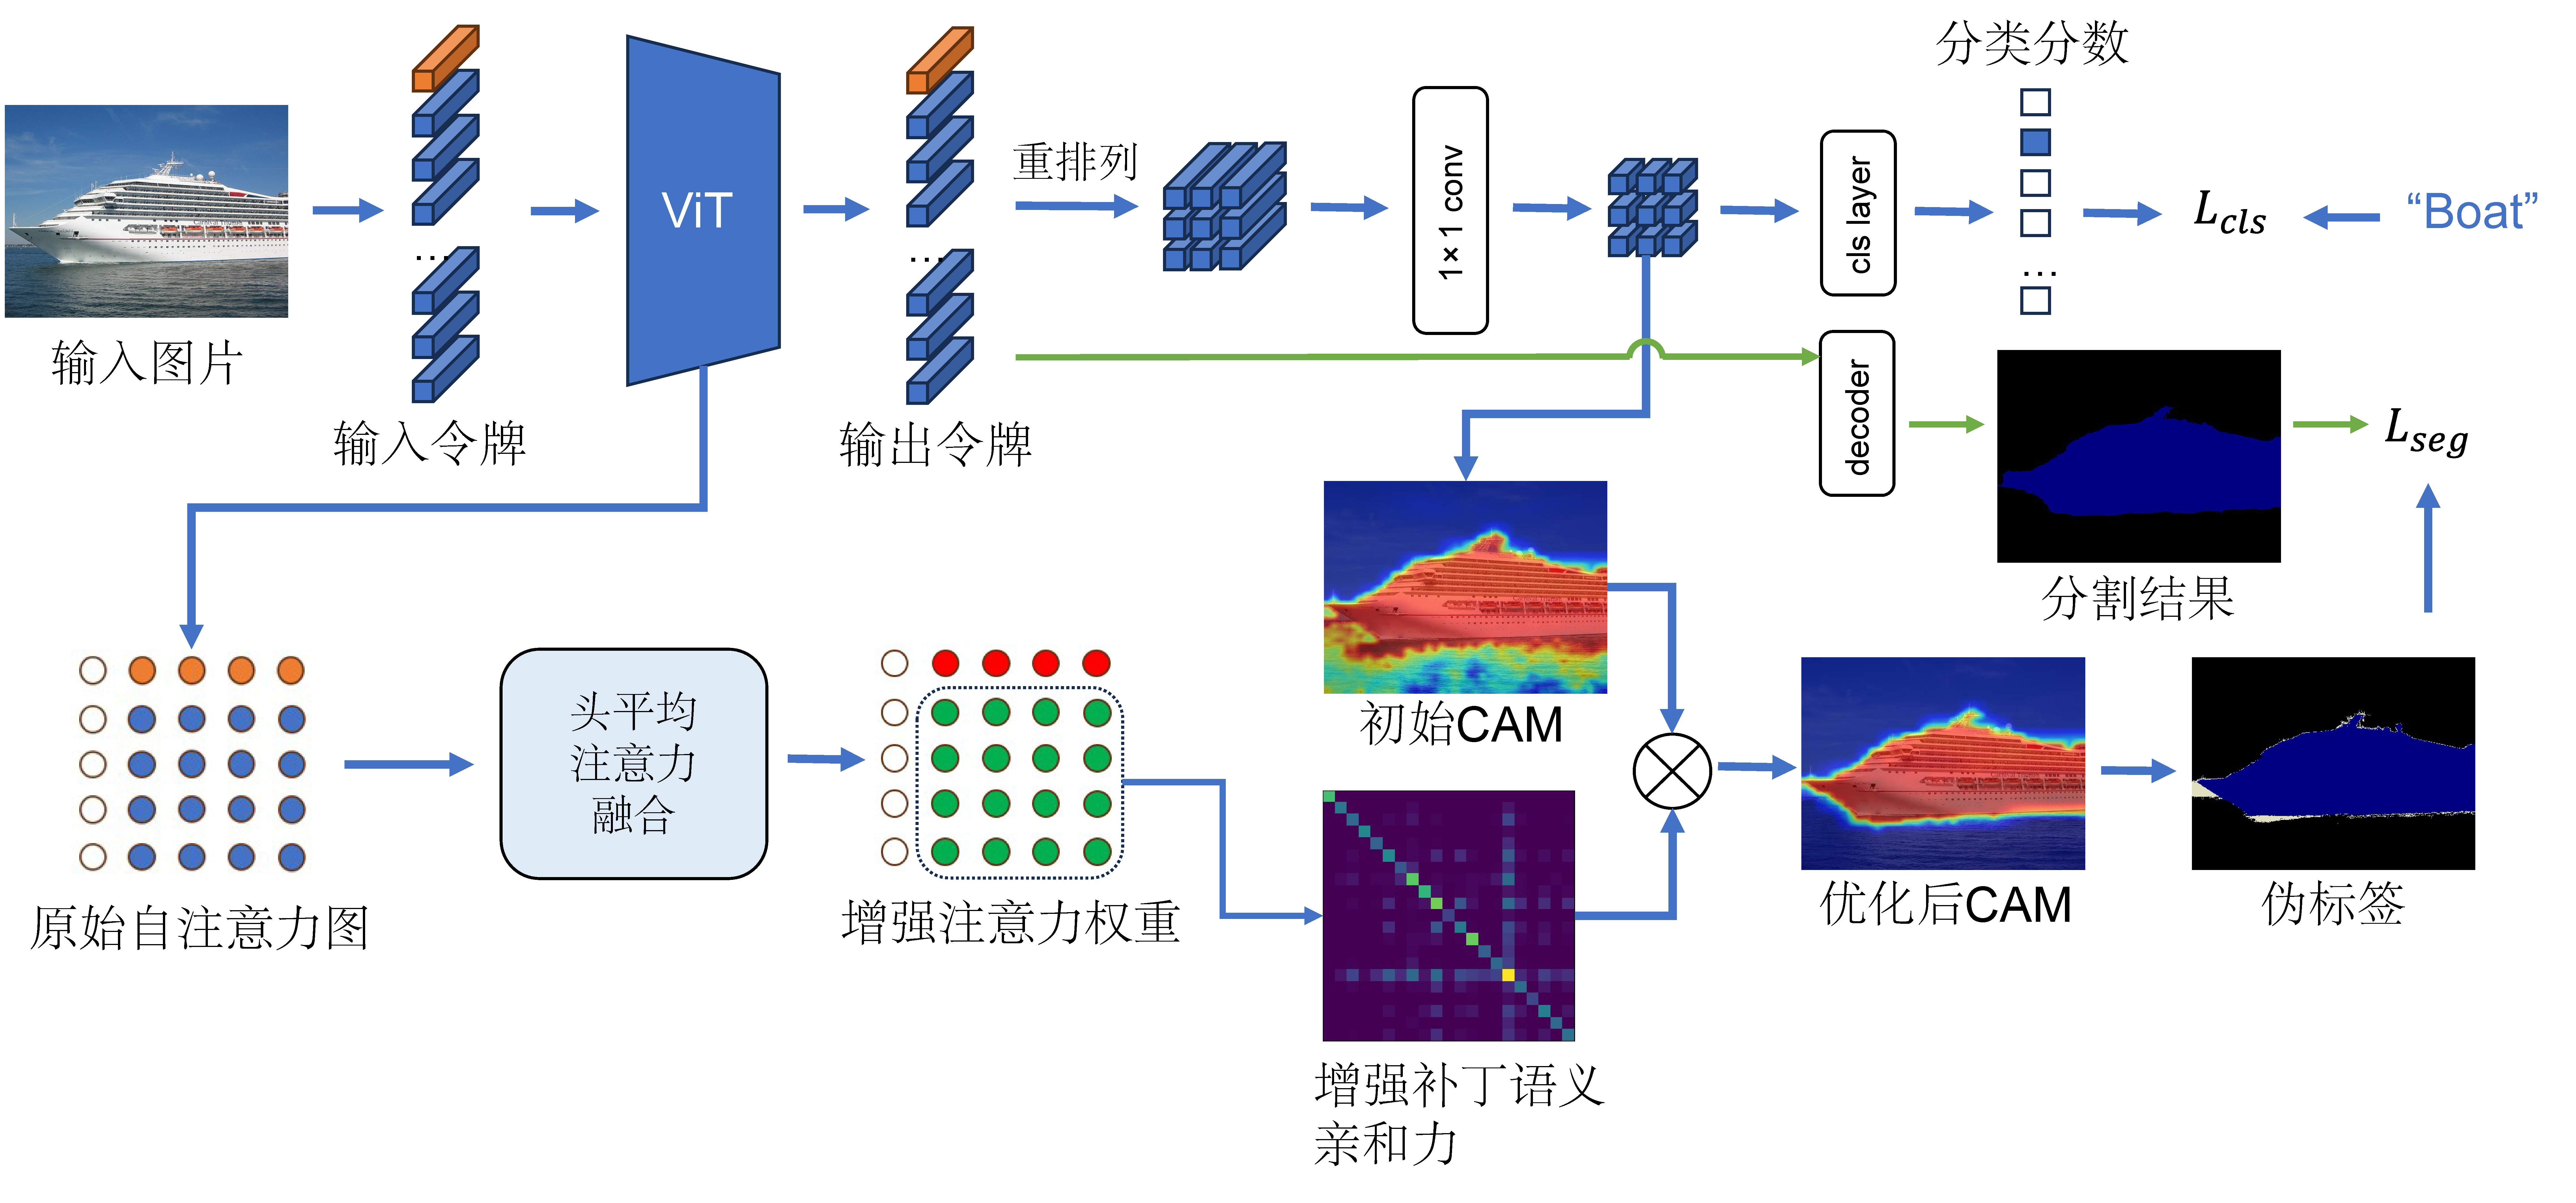
\includegraphics[width=6in]{fig/fig1.pdf}}
%     \begin{CJK*}{UTF8}{fs}
%         \caption{SS-EPA整体框架。SS-EPA首先将输入图像分成多个补丁,每个补丁线性转换成补丁令牌,并连接一个类别令牌。ViT输出令牌一方面经过重拍列和$1\times 1$卷积生成初始CAM,并由分类层输出分类分数。另一方面经过分割decoder生成语义分割结果。然后从ViT中提取多头自注意力图,并通过HAAF模块进行增强,获取增强补丁语义亲和力。最后通过增强补丁语义亲和力对初始CAM进行优化,并生成伪标签用于监督分割任务。}\label{fig1}
%     \end{CJK*}
% \end{figure*}

\vspace{2mm}

\begin{CJK*}{UTF8}{zhhei}
    \subsection{SS-EPA框架}\label{section3.2}
\end{CJK*}





SS-EPA首先将输入图片拆分为 $N\times N$ 个补丁,并通过线性转换为补丁令牌序列 $T_{\text{patch}}\in R^{N^2\times D}$,其中D是嵌入维度。
生成一个维度同样为D的类令牌 $T_{\text{cls}}\in R^{1\times D}$,将类令牌与补丁令牌链接,并添加位置编码构成ViT编码器的输入令牌序列 $T_{\text{input}}\in R^{(1+N^2)\times D}$。
ViT backbone具有$K$个Transformer编码层,每个编码层包含一个多头自注意力和一个多层感知机,以及分别用于两个子层前的层归一化。
ViT编码器接收输入令牌序列$T_{\text{input}}^i,i=(1,2,…,K)$,并输出令牌序列$T_{\text{out}}^i\in R^{(1+N^2)\times D},i=(1,2,…,K)$。
最后一层Transformer编码层的输出令牌序列$T_{\text{out}}^K\in R^{(1+N^2)\times D}$,去除类令牌对应维度并重排列可得补丁令牌序列$T_{\text{out\_patch}}\in R^{N\times N\times D}$,并执行$1\times 1$卷积操作将令牌维度变为物体类别数量,公式如下:

\begin{equation}
    \text{CAM}=\text{conv}_{1\times 1} (T_\text{out\_patch})
\end{equation}
其中,$\text{conv}_{1\times 1}$的输入通道为D,输出通道为物体类别数$C$,卷积核大小为$1\times 1$。通过上式可获得来自补丁令牌的初始类激活图$\text{CAM}\in R^{N\times N\times C}$。参照\cite{13ru2022learning}的方法,通过一个全局最大池化层(Global Max Pooling)来聚合补丁令牌$T_{\text{out\_patch}}$信息,然后通过全连接层来计算分类分数cls\_score,分类损失函数使用多标签软边距损失(Multi Label Soft Margin Loss)作为损失函数$L_{cls}$,公式如下:
\begin{equation}
    \begin{aligned}
        L_\text{cls}(x,y) = - \frac{1}{C}&\sum_{i=1}^C [y\log(\sigma (x)) \\
        &+(1-y)\log(1-\sigma (x))]
    \end{aligned}
\end{equation}
其中$x$,$y$分别是模型预测分数与真值标签,$\sigma(x)$表示Sigmoid函数的输出,即:
\begin{equation}
    \sigma(x) = \frac{1}{1+e^{-x}}
\end{equation}

ViT backbone使用的是标准的 Transformer 多头自注意力,首先将输入令牌归一化,并通过全连接层将其转换为一个查询$Q\in R^{(1+N^2)\times D}$和一组键值$K\in R^{(1+N^2)\times D}$、$V\times R^{(1+N^2)\times D}$,注意力计算采用\cite{14vaswani2017attention}中的缩放点积注意力(Scaled Dot-Product Attention),计算公式如下:

\begin{equation}
    \text{Attn}(Q,K,V)=\left(\text{Softmax}\frac{QK^T}{\sqrt{D}}\right)V
\end{equation}
从中可以提取多头自注意力图$A_{map}=QK^T$,其中$A_{\text{map}}^i\in R^{H\times (1+N^2)\times (1+N^2)} ,i=1,\cdots,K$,$H$为多头自注意力头的个数。此操作不会带来任何额外的计算资源消耗,因为多头自注意力权重是Transformer在计算时产生的副产物。然后在第$0$个维度上进行concatenate操作将$K$层注意力图串联起来,获得全局注意力张量$A\in R^{K\times H\times (1+N^2)\times (1+N^2)}$,该注意力张量十分庞大,在\ref{section3.3_HAAF}节中将讨论如何减小计算资源占用。

% \begin{figure*}[htbp]
%     \centerline{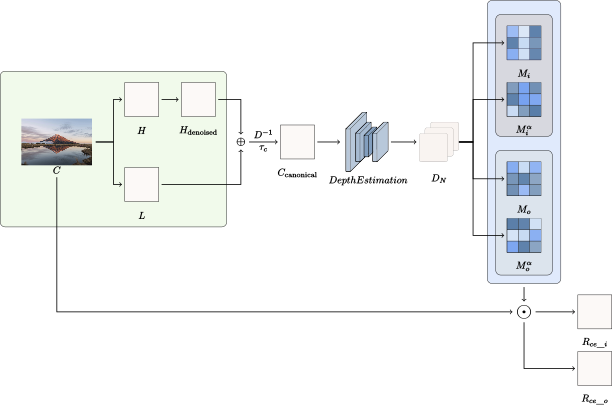
\includegraphics[width=6in]{fig/fig2.pdf}}
%     \begin{CJK*}{UTF8}{fs}
%         \caption{补丁语义亲和力获取流程图}\label{fig2}
%     \end{CJK*}
% \end{figure*}

全局注意力张量$A$中蕴含了补丁语义亲和力信息,将注意力图$A$在第$0$和第$1$个维度上进行平均来聚合来自不同层和不同头的注意力信息,得到$A_{\text{fused}}\in R^{(1+N^2)\times (1+N^2)}$,除去其中类令牌对应的维度,如图\ref{fig2}所示,剩下的注意力权重可作为补丁级语义亲和力$\text{PatchAffinity}\in R^{N^2 \times N^2}$。由于从补丁令牌生成的初始类激活图CAM存在大量噪声与错误,所以需要补丁级语义亲和力对其进行优化,优化公式如下:

\begin{equation}
    \text{CAM}_{\text{refined}}=\text{PatchAffinity}\times \text{CAM}
\end{equation}

通过上式可获得通过原始补丁语义亲和力优化后的类激活图$\text{CAM}_\text{refined}\in R^{N\times N\times C}$,相比初始CAM对目标的覆盖性更好,错误激活区域更少,且可以激活更多目标区域。


\vspace{2mm}


\begin{CJK*}{UTF8}{zhhei}
    \subsection{头平均注意力融合增强模块(HAAF)}
    \label{section3.3_HAAF}
\end{CJK*}

鉴于 Transformer 中不同深度的层的多头自注意力可能关注不同部分,如浅层更关注局部结构、纹理颜色等,深层能捕获更广泛和抽象的视觉语义信息,所以不能简单地将来自不同层的多头自注意力平均来聚合语义信息。
且一个标准ViT backbone(vit\_base\_patch16\_224)的多头自注意力图十分庞大(batchsize为2时,显存占用超过12GB),对计算资源要求较高。
本文提出头平均注意力融合增强模块(HAAF)来解决上述问题,如图\ref{fig3}所示。

\begin{figure}[htbp]
    \centerline{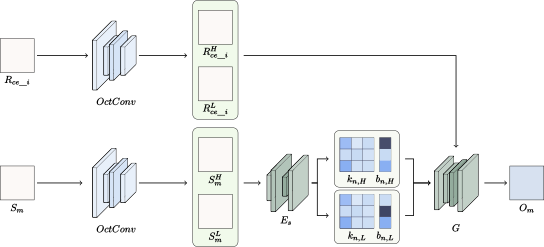
\includegraphics[width=3.15in]{fig/fig3.pdf}}
    \begin{CJK*}{UTF8}{fs}
        \caption{HAAF结构图}\label{fig3}
    \end{CJK*}
\end{figure}

\begin{figure*}[t]
    \centerline{
\includegraphics[width=6in]{fig/fig4.pdf}}
    \begin{CJK*}{UTF8}{fs}
        \caption{增强补丁语义亲和力获取流程图}\label{fig4}
    \end{CJK*}
\end{figure*}

对于\ref{section3.2}节中从backbone中提取的多头自注意力图$A_\text{map}^i\in R^{H\times (1+N^2)\times (1+N^2)},i=1,…,K$,HAAF首先采用头平均操作去除维度$H$,有助于去除冗余信息并减少$H$倍的显存占用,得到$A_\text{mean\_head}^i\in R^{(1+N^2)\times (1+N^2)},i=1,…,K$。
然后在第$0$个维度上进行concatenate操作将$K$层注意力图串联起来,获得全局注意力张量$A'\in R^(K\times (1+N^2)\times (1+N^2) )$。全局平均池化通过平滑特征表示和增强泛化能力,相较于全局最大池化,在减少噪声和防止过拟合方面更具优势。
所以本文通过全局平均池化聚合K层注意力图的全局特征,得到聚合后的长度为$K$的特征向量$V\in R^{K\times 1\times 1}$,并将特征向量输入多层感知机中相互作用,提取更复杂的特征相互关系,多层感知机输出相同形状的特征向量$V'\in R^(K\times 1\times 1)$。获得多层感知机输出的特征向量$V'$后,将全局注意力张量$A'$与特征向量$V'$结合,公式如下:
\begin{equation}
    A'_\text{enhanced} = A' \odot V'
\end{equation}
其中$\odot$表示逐元素相乘符号。
通过上式可获得充分考虑了不同层注意力重要性的增强注意力图$A_\text{enhanced}'\in R^{K\times (1+N^2)\times (1+N^2)}$。经过头平均后的注意力图更加稳定,不易受到单个注意力头学习偏差的影响。



% \begin{figure*}[htbp]
%     \centerline{
\includegraphics[width=6in]{fig/fig4.pdf}}
%     \begin{CJK*}{UTF8}{fs}
%         \caption{增强补丁语义亲和力获取流程图}\label{fig4}
%     \end{CJK*}
% \end{figure*}

图\ref{fig4}展示了不同层增强注意力图的融合过程,对增强注意力图$A_\text{enhanced}'$在第$0$个维度$K$上进行平均操作,可得到融合增强注意力$A_\text{fused}'\in R^{(1+N^2)\times (1+N^2)}$。
除去其中类令牌对应的维度,剩下的增强注意力权重可作为增强后的补丁级语义亲和力$\text{PA}_\text{enhanced}\in R^{N^2\times N^2}$,如图\ref{fig4}所示。通过HAAF增强后的补丁语义亲和力$\text{PA}_\text{enhanced}$相比增强前减少了噪声与错误,并且充分考虑了不同层注意力的重要性。通过特征向量$V'$对每层注意力进行加权。最后利用$\text{PA}_\text{enhanced}$对CAM优化,过程与3.2节介绍的CAM优化过程类似,优化公式如下:

\begin{equation}
\text{CAM}'_\text{refined} = \text{PA}_\text{enhanced} \times CAM
\end{equation}
其中$\text{CAM}$是来自补丁令牌的初始类激活图$\text{CAM}\in R^{N\times N\times C}$,通过上式可获得通过增强补丁语义亲和力优化后的类激活图$\text{CAM}_\text{refined}'\in R^(N\times N\times C)$。$\text{CAM}_\text{refined}'$相比直接利用语义亲和力优化的$\text{CAM}_\text{refined}$,拥有更全面的激活区域和更精细的对象边界,且有更高的鲁棒性。

\vspace{2mm}
\begin{CJK*}{UTF8}{zhhei}
    \subsection{模型训练与损失函数}
\end{CJK*}

如图\ref{fig1}所示,使用多标签软边缘损失作为分类损失$L_\text{cls}$,使用交叉熵损失作为分割损失$L_\text{seg}$。参照基线方法ToCo[3],本文使用了辅助分类损失$L_\text{m\_cls}$,以及令牌对比损失$L_\text{ptc}$和$L_\text{ctc}$。此外,为了进一步提高性能,还按照先前的方法\cite{13ru2022learning,15tang2018regularized,16zhang2021dynamic,17zhang2020reliability},采用了正则化损失$L_\text{reg}$,所以SS-EPA的损失最终定义如下:

\begin{equation}
    \begin{aligned}
        L=&L_\text{cls}+\lambda_1 L_\text{seg}+\lambda_2 L_\text{m\_cls}\\
        &+\lambda_3 L_\text{ptc}+ \lambda_4 L_\text{ctc}+ \lambda_5 L_\text{reg}
    \label{equation_8}
    \end{aligned}
\end{equation}
其中,超参数$\lambda_i,i=1,2,\cdots,5$用于平衡不同损失的权重。
%添加方法论
\begin{CJK*}{UTF8}{zhhei}
    \zihao{5}
    \vskip 1mm
    \section{实验}
\end{CJK*}


\begin{CJK*}{UTF8}{zhhei}
    \subsection{实验设置}
\end{CJK*}

\begin{CJK*}{UTF8}{zhhei}
    \subsubsection{数据集}
\end{CJK*}
本文在Pascal VOC 2012\cite{18everingham2010pascal}数据集上评估所提方法。Pascal VOC 2012包含20个前景类别和1个背景类别。它有三个子集:训练集(train)、验证集(val)和测试集(test),分别包含1464、1449 和 1456张图片。按照先前方法\cite{06wang2020self,12xu2022multi,13ru2022learning,03ru2023token}的常用做法,本文进一步利用SBD数据集将VOC训练集图片数量扩充至10582。在训练过程中,本文严格只使用图像级分类标签用于监督模型训练。

\begin{CJK*}{UTF8}{zhhei}
    \subsubsection{评估指标}
\end{CJK*}
与先前方法一样,本文使用平均交并比(mean Intersection over Union,mIoU),作为CAM质量、伪标签质量以及语义分割模型性能的评估指标。本文方法在Pascal VOC测试集上的评估结果由官方在线评估服务器给出。

\begin{CJK*}{UTF8}{zhhei}
    \subsubsection{实现细节}
\end{CJK*}

\begin{figure*}[t]
    \centerline{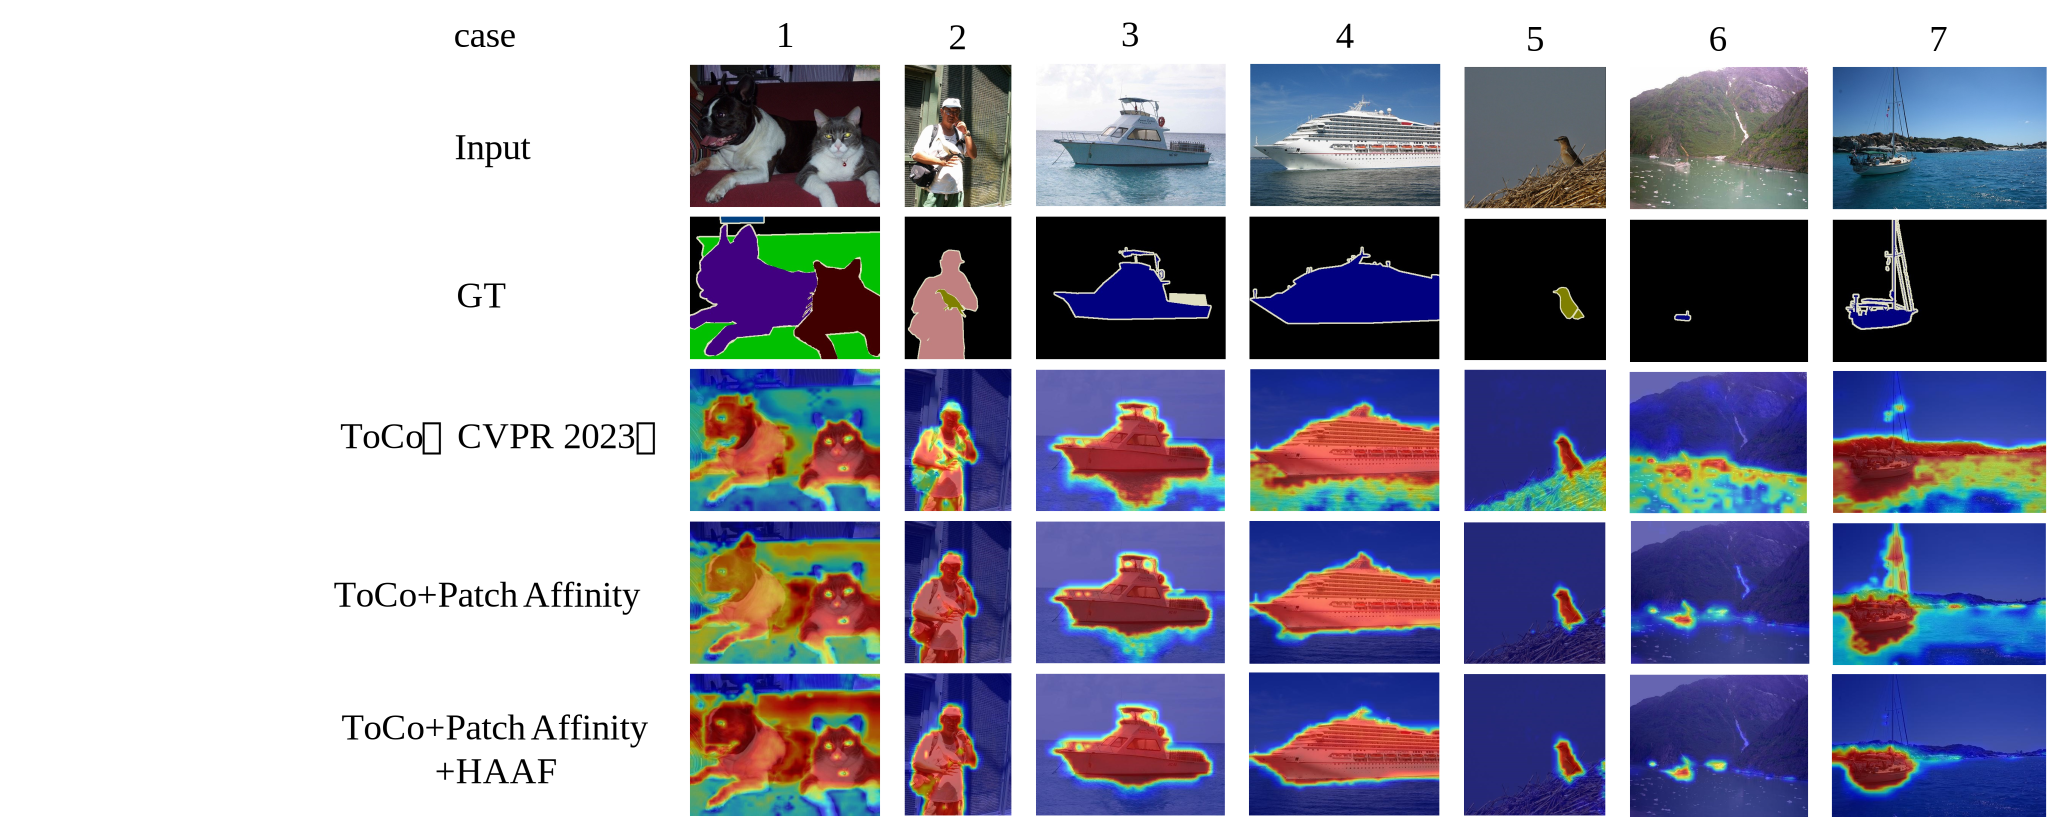
\includegraphics[width=6in]{fig/fig5.pdf}}
    \begin{CJK*}{UTF8}{fs}
        \caption{生成CAM可视化结果,从上到下依次为输入图片(input),真值标签(GT),ToCo生成CAM,SS-EPA生成CAM(不使用HAAF),SS-EPA生成CAM(使用HAAF)。红框部分为显著提升区域。}\label{fig5}
    \end{CJK*}
\end{figure*}

本文利用在 ImageNet 数据集\cite{19deng2009imagenet}上预训练的ViT-B(vit\_base\_patch16\_224)\cite{02dosovitskiy2020image}作为 backbone,它有$12$层 Transformer 编码层,$12$个注意力头,嵌入维度为$768$。卷积解码器使用 LargeFOV \cite{20chen2017deeplab},它由两个膨胀系数为$5$的$3\times 3$卷积和一个$1\times 1$卷积预测层构成。

输入图片被随机裁剪为$448\times 448$的大小。模型共训练$20000$个迭代,batch-size设置为$4$,模型优化器采用AdamW\cite{21loshchilov2017decoupled},学习率在前$1500$个迭代中逐渐提升到$6\times 10^{-5}$,并在后续根据多项式调度器衰减。公式\ref{equation_8}中的权重因子$\lambda_i,i=1,2,…,5$在前$2000$个迭代分别设置为($0, 1.0, 0.2, 0.5, 0$),$2000$个迭代后分别设置为($0.1, 1.0, 0.2, 0.5, 0.05$)。

\vspace{2mm}

\begin{CJK*}{UTF8}{zhhei}
    \subsection{实验结果}
\end{CJK*}
\begin{CJK*}{UTF8}{zhhei}
    \subsubsection{CAM与伪标签}
\end{CJK*}

\begin{table}[t]
    \setlength{\tabcolsep}{4mm}
    \tiny
    \centering
    \caption{伪标签生成定量评估(MS:Multi Scale,CRF:dense CRF)(单位mIoU\%)}\label{table1}
    \begin{tabular}{lccc}
        \toprule
        Method & Backbone & train & val \\
        \midrule
        \textbf{\textit{Multi-Stage WSSS Methods}}& & &\\
        ViT-PCM\cite{23rossetti2022max}	& ViT-B & 67.7 & 66.0\\
        MCTformer\cite{12xu2022multi} & Deit-S & 69.1 & -\\
        LPCAM\cite{24chen2023extracting} & Deit-S & - & 70.8\\
        SFC\cite{26zhao2024sfc} & ResNet101 & 73.7 & -\\
        POLE\cite{25murugesan2024prompting} & ResNet50 & 74.2 & -\\
        \cmidrule[0.4pt](lr){1-4}
        \textbf{\textit{Single-Stage WSSS Methods}}& & &\\
        RRM\cite{17zhang2020reliability} & ResNet38 & - & 65.4\\
        1Stage\cite{27araslanov2020single} & ResNet38 & 66.9 & 65.3\\
        SLRNet\cite{28pan2022learning} & ResNet38 & 67.1 & 66.2\\
        AFA\cite{13ru2022learning} & MiT-B1 & 68.7 & 66.5\\
        MCC\cite{29wu2024masked} & Deit-B & 75.1 & 72.2\\
        ToCo\cite{03ru2023token} & ViT-B & 74.5 & 72.2\\
        ToCo+MS+CRF\cite{03ru2023token} & ViT-B & 77.3 & 74.6\\
        \textbf{SSEPA} & \textbf{ViT-B} & \textbf{77.1} & \textbf{74.2}\\
        \bottomrule
    \end{tabular}
\end{table}

图\ref{fig5}呈现了SS-EPA生成CAM的可视化结果,并与基线模型ToCo相比较。可以看出,SS-EPA在不使用HAAF的情况下,生成的CAM比ToCo更少,说明利用原始补丁语义亲和力优化CAM,可以显著减少初始CAM中的噪声,纠正错误激活的背景区域,使CAM更加精准和细化。在使用HAAF后,SS-EPA可能够发现一些未被初始CAM激活的前景区域(如图\ref{fig5}中case~1与case~2),并生成错误更少的CAM(如图\ref{fig5}中case~3至case~7),这说明了本文提出的HAAF可以进一步优化补丁语义亲和力,从而生成更优质的CAM。

% \begin{figure*}[htbp]
%     \centerline{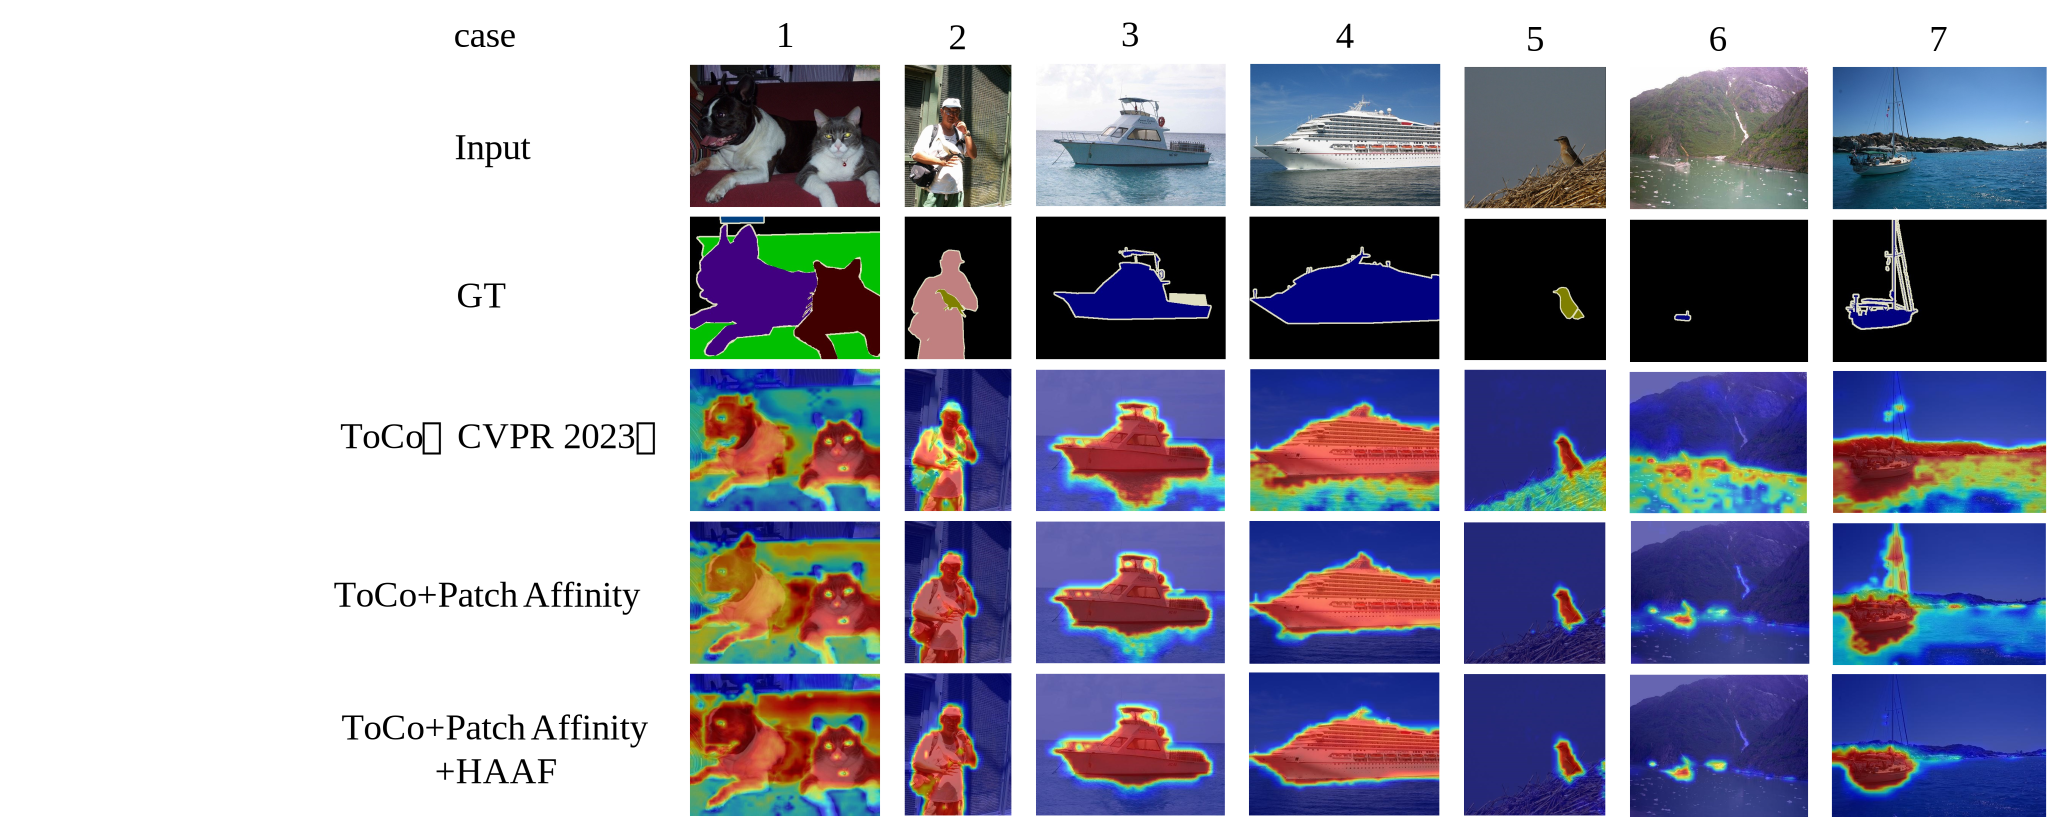
\includegraphics[width=6in]{fig/fig5.pdf}}
%     \begin{CJK*}{UTF8}{fs}
%         \caption{生成CAM可视化结果,从上到下依次为输入图片(input),真值标签(GT),ToCo生成CAM,SS-EPA生成CAM(不使用HAAF),SS-EPA生成CAM(使用HAAF)。红框部分为显著提升区域。}\label{fig5}
%     \end{CJK*}
% \end{figure*}

表\ref{table1}呈现了利用 CAM 生成伪标签的定量评估结果,在 VOC 训练集和验证集上进行评估,并与一些先进的 WSSS 方法进行比较。结果表明,本文提出的 SS-EPA 比现有的单阶段 WSSS 方法更好,且达到了与一些多阶段 WSSS 方法相当的性能。与基线方法 ToCo 相比较,无论是否使用 MS(Multi Scale) 和 CRF(DenseCRF) , SS-EPA 的性能都要优于 ToCo 。

% \begin{table}[t]
%     \setlength{\tabcolsep}{4mm}
%     \tiny
%     \centering
%     \caption{伪标签生成定量评估(MS:Multi Scale,CRF:dense CRF)(单位mIoU\%)}\label{table1}
%     \begin{tabular}{lccc}
%         \toprule
%         Method & Backbone & train & val \\
%         \midrule
%         \textbf{\textit{Multi-Stage WSSS Methods}}& & &\\
%         ViT-PCM\cite{23rossetti2022max}	& ViT-B & 67.7 & 66.0\\
%         MCTformer\cite{12xu2022multi} & Deit-S & 69.1 & -\\
%         LPCAM\cite{24chen2023extracting} & Deit-S & - & 70.8\\
%         SFC\cite{26zhao2024sfc} & ResNet101 & 73.7 & -\\
%         POLE\cite{25murugesan2024prompting} & ResNet50 & 74.2 & -\\
%         \cmidrule[0.4pt](lr){1-4}
%         \textbf{\textit{Single-Stage WSSS Methods}}& & &\\
%         RRM\cite{17zhang2020reliability} & ResNet38 & - & 65.4\\
%         1Stage\cite{27araslanov2020single} & ResNet38 & 66.9 & 65.3\\
%         SLRNet\cite{28pan2022learning} & ResNet38 & 67.1 & 66.2\\
%         AFA\cite{13ru2022learning} & MiT-B1 & 68.7 & 66.5\\
%         MCC\cite{29wu2024masked} & Deit-B & 75.1 & 72.2\\
%         ToCo\cite{03ru2023token} & ViT-B & 74.5 & 72.2\\
%         ToCo+MS+CRF\cite{03ru2023token} & ViT-B & 77.3 & 74.6\\
%         \textbf{SSEPA} & \textbf{ViT-B} & \textbf{77.1} & \textbf{74.2}\\
%         \bottomrule
%     \end{tabular}
% \end{table}
\begin{figure*}[htbp]
    \centerline{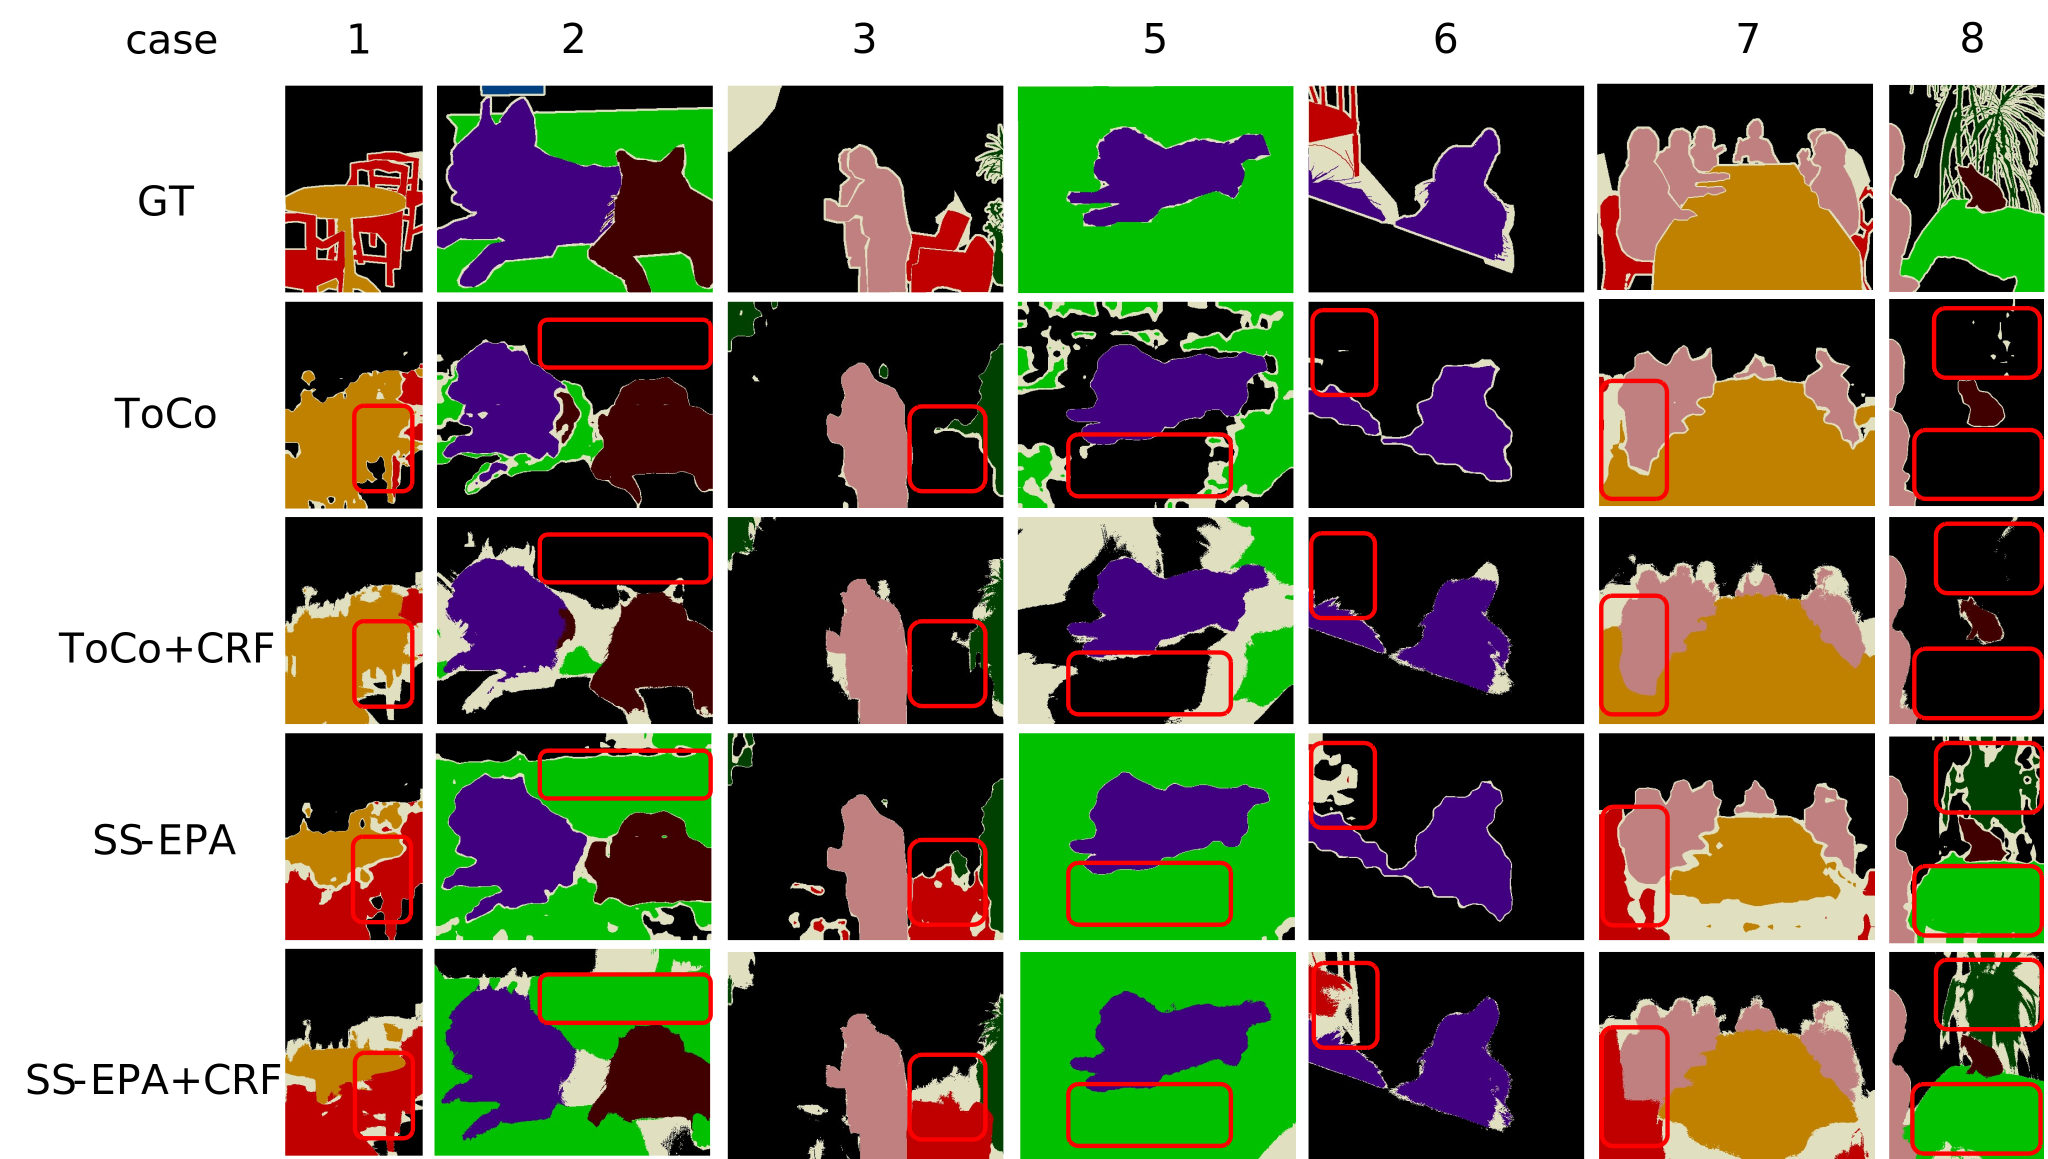
\includegraphics[width=6in]{fig/fig6.pdf}}
    \begin{CJK*}{UTF8}{fs}
        \caption{生成伪标签的可视化结果,从上到下依次为分割真值标签(GT),ToCo分割结果(不加CRF),ToCo分割结果(加CRF),SS-EPA分割结果(不加CRF),SS-EPA分割结果(加CRF)。红框部分为显著提升区域。}\label{fig6}
    \end{CJK*}
\end{figure*}

\begin{table}[htbp]
    
    \normalsize
    \setlength{\tabcolsep}{4mm}
    \centering
    \caption{分割结果定量评估(单位mIoU\%)}\label{table2}
    \tiny
    \begin{tabular}{lccc}
        \toprule
        Method & Backbone & train & val \\
        \midrule
        \textbf{\textit{Multi-Stage WSSS Methods}}& & &\\
        ReCAM\cite{33chen2022class} & ResNet101 & 68.5 & 68.4\\
        ViT-PCM\cite{23rossetti2022max }& ResNet101 & 70.3 & 70.9\\
        CLIMS\cite{08xie2022clims} & ResNet101 & 70.4 & 70.0\\
        AMN\cite{34lee2022threshold} & ResNet101 & 70.7 & 70.6\\
        EDAM\cite{30wu2021embedded} & ResNet101 & 70.9 & 70.6 \\
        SFC\cite{26zhao2024sfc} & ResNet101 & 71.2 & 72.5 \\
        POLE\cite{25murugesan2024prompting} & ResNet50 & 71.5 & 71.4 \\
        MCTformer\cite{12xu2022multi} & Deit-S & 71.9 & 71.6 \\
        L2G\cite{31jiang2022l2g} & ResNet101 & 72.1 & 71.7 \\
        BECO\cite{35rong2023boundary} & ResNet101 & 72.1 & 71.8 \\
        RCA\cite{32zhou2022regional} & ResNet38 & 72.2 & 72.8 \\
        LPCAM\cite{24chen2023extracting} & Deit-S & 72.6 & 72.4 \\
        OCR\cite{36cheng2023out} & ResNet38 & 72.7 & 72.0 \\
        \cmidrule[0.4pt](lr){1-4}
        \textbf{\textit{Single-Stage WSSS Methods}}& & &\\
        RRM\cite{27araslanov2020single} & ResNet38 & 62.6 & 62.9 \\
        1Stage\cite{27araslanov2020single} & ResNet38 & 62.7 & 64.3 \\
        AFA\cite{13ru2022learning} & MiT-B1 & 66.0 & 66.3 \\
        SLRNet\cite{28pan2022learning} & ResNet38 & 67.2 & 67.6 \\
        MCC\cite{29wu2024masked} & Deit-B & 70.3 & 71.2 \\
        ToCo\cite{03ru2023token} & ViT-B & 71.1 & 72.2 \\
        \textbf{SSEPA} & \textbf{ViT-B} & \textbf{72.4} & \textbf{73.2}\\
        \bottomrule
    \end{tabular}
\end{table}

图\ref{fig6}是 SS-EPA 生成伪标签的可视化结果,包括使用 DenseCRF\cite{22chen2014semantic} 后处理前后的结果。可视化结果表明,无论是否使用 CRF,SS-EPA 生成的伪标签在准确度上都高于 ToCo(如图6中 case 1 与case 7),且能识别到一些 ToCo 无法识别到的目标(如图6中 case 2 至 case 6 )。



\begin{CJK*}{UTF8}{zhhei}
    \subsubsection{分割结果}
\end{CJK*}

表\ref{table2}中呈现了在 Pascal VOC 2012 数据集上的定量语义分割结果,比较了本文提出的 SS-EPA 与其它的 WSSS 方法在 mIoU 分数上的表现。 SS-EPA 用ImageNet 预训练的 ViT-B(vit\_base\_patch16\_224) 作为b ackbone,在验证集和测集上分别达到了 72.4\% 和 73.3\% 的mIoU分数,比基线方法 ToCo 提升了 1.3\% 和 1.1\% 的 mIoU 分数。结果表明, SS-EPA 的性能优于现有的利用图像级标签的单阶段 WSSS 方法。此外,SS-EPA 与许多多阶段 WSSS 方法的性能相当,证明了本文所提方法的有效性。


% \begin{table}[htbp]
    
%     \normalsize
%     \setlength{\tabcolsep}{4mm}
%     \centering
%     \caption{分割结果定量评估(单位mIoU\%)}\label{table2}
%     \tiny
%     \begin{tabular}{lccc}
%         \toprule
%         Method & Backbone & train & val \\
%         \midrule
%         \textbf{\textit{Multi-Stage WSSS Methods}}& & &\\
%         ReCAM\cite{33chen2022class} & ResNet101 & 68.5 & 68.4\\
%         ViT-PCM\cite{23rossetti2022max }& ResNet101 & 70.3 & 70.9\\
%         CLIMS\cite{08xie2022clims} & ResNet101 & 70.4 & 70.0\\
%         AMN\cite{34lee2022threshold} & ResNet101 & 70.7 & 70.6\\
%         EDAM\cite{30wu2021embedded} & ResNet101 & 70.9 & 70.6 \\
%         SFC\cite{26zhao2024sfc} & ResNet101 & 71.2 & 72.5 \\
%         POLE\cite{25murugesan2024prompting} & ResNet50 & 71.5 & 71.4 \\
%         MCTformer\cite{12xu2022multi} & Deit-S & 71.9 & 71.6 \\
%         L2G\cite{31jiang2022l2g} & ResNet101 & 72.1 & 71.7 \\
%         BECO\cite{35rong2023boundary} & ResNet101 & 72.1 & 71.8 \\
%         RCA\cite{32zhou2022regional} & ResNet38 & 72.2 & 72.8 \\
%         LPCAM\cite{24chen2023extracting} & Deit-S & 72.6 & 72.4 \\
%         OCR\cite{36cheng2023out} & ResNet38 & 72.7 & 72.0 \\
%         \cmidrule[0.4pt](lr){1-4}
%         \textbf{\textit{Single-Stage WSSS Methods}}& & &\\
%         RRM\cite{27araslanov2020single} & ResNet38 & 62.6 & 62.9 \\
%         1Stage\cite{27araslanov2020single} & ResNet38 & 62.7 & 64.3 \\
%         AFA\cite{13ru2022learning} & MiT-B1 & 66.0 & 66.3 \\
%         SLRNet\cite{28pan2022learning} & ResNet38 & 67.2 & 67.6 \\
%         MCC\cite{29wu2024masked} & Deit-B & 70.3 & 71.2 \\
%         ToCo\cite{03ru2023token} & ViT-B & 71.1 & 72.2 \\
%         \textbf{SSEPA} & \textbf{ViT-B} & \textbf{72.4} & \textbf{73.2}\\
%         \bottomrule
%     \end{tabular}
% \end{table}


图\ref{fig7}展示了SS-EPA、ToCo和真实标签的分割结果。可视化结果表明,本文提出的SS-EPA成功分割了图像中的多个对象,并且与ToCo相比,SS-EPA分类的准确度更高(如图7中Val的case 1、3、4,Test的case 5、7、8),能正确发现一些ToCo中误分类为背景的前景目标(如图7中Val的case 2,Test的case 6),且整体对象边界都更加完整和准确。

\begin{figure*}[htbp]
    \centerline{\includegraphics[width=6in]{fig/fig7_h.pdf}}
    \begin{CJK*}{UTF8}{fs}
        \caption{分割结果的可视化结果,左半部分为VOC验证集(Val),从上到下依次为输入图片(input),分割真值标签(GT),ToCo分割结果,SS-EPA分割结果。右半部分为VOC测试集(Test),从上到下依次为输入图片(input),ToCo分割结果,SS-EPA分割结果。红框部分为显著提升区域。}\label{fig7}
    \end{CJK*}
\end{figure*}


\vspace{2mm}

\begin{CJK*}{UTF8}{zhhei}
    \subsection{消融实验}
\end{CJK*}

% \begin{table*}[!htbp]
%     \small
%     \setlength{\tabcolsep}{6mm}
%     \centering
%     \caption{分割结果定量评估(单位mIoU\%)}\label{table3}
%     \begin{tabular}{lccc}
%         \toprule
%         Method & Pseudo label(train) & Seg(val) & Seg(test) \\
%         \midrule
%         ToCo & 77.3 & 71.1 & 72.21 \\
%         SS-EPA(w/o Patch Affinity) & 76.2 & 71.3 & 71.62 \\
%         SS-EPA(with Patch Affinity) & 79.0 & 71.9 & 72.73 \\
%         \textbf{SS-EPA(with Patch Affinity HAAF)} & \textbf{79.5} & \textbf{72.4} & \textbf{73.34} \\  
%         \bottomrule
%     \end{tabular}
% \end{table*}


\begin{CJK*}{UTF8}{zhhei}
    \subsubsection{补丁语义亲和力分析}
\end{CJK*}

表\ref{table3}呈现了关于伪标签和分割结果的消融实验定量评估。结果表明,使用不加HAAF增强的补丁语义亲和力后,SS-EPA可以生成更加优质的伪标签并提高分割性能。其中伪标签提升了2.8\%,分割性能在验证集和测试集上分别提升了0.6\%和1.1\%,分割的准确率更高。从图5可看出尽管在未使用HAAF的情况下存在噪声与错误,补丁语义亲和力仍有效优化了初始 CAM。

\begin{table}[!htbp]
    % \setlength{\tabcolsep}{6mm}
    \centering
    \caption{分割结果定量评估(单位mIoU\%)}\label{table3}
    \tiny
    \begin{tabular}{lccc}
        \toprule
        Method & Pseudo label(train) & Seg(val) & Seg(test) \\
        \midrule
        ToCo & 77.3 & 71.1 & 72.21 \\
        SS-EPA(w/o Patch Affinity) & 76.2 & 71.3 & 71.62 \\
        SS-EPA(with Patch Affinity) & 79.0 & 71.9 & 72.73 \\
        \textbf{SS-EPA(with Patch Affinity HAAF)} & \textbf{79.5} & \textbf{72.4} & \textbf{73.34} \\  
        \bottomrule
    \end{tabular}
\end{table}

\begin{CJK*}{UTF8}{zhhei}
    \subsubsection{HAAF分析}
\end{CJK*}

如\ref{section3.3_HAAF}节中所说,补丁语义亲和力存在噪声与错误,直接使用补丁语义亲和力并不合适。本文提出的HAAF模块显著减少了语义亲和力中的噪声和错误,并减少计算资源占用。从表3中可以看出,HAAF进一步提升了伪标签和分割结果的mIoU分数,其中伪标签提升了0.5\%,分割性能在验证集和测试集上分别提升了0.5\%和0.6\%。

\begin{table}[!htbp]
    % \setlength{\tabcolsep}{7mm}
    \centering
    \caption{SS-EPA计算资源占用实验结果评估(单位GB)}\label{table4}
    \tiny
    \begin{tabular}{lccc}
        \toprule
        Method & Backbone & Batchsize 1 & Batchsize 2 \\
        \midrule
        SS-EPA(w/o Patch Affinity) & ViT-B & 6.6 & 10.4 \\
        SS-EPA(with Patch Affinity) & ViT-B & 13.2 & 23.6 \\
        \textbf{SS-EPA(with Patch Affinity HAAF)} & \textbf{ViT-B} & \textbf{8.3} & \textbf{12.6} \\  
        \bottomrule
    \end{tabular}
\end{table}

表\ref{table4}展示了 SS-EPA 的计算资源占用评估,分别评估了 batchsize~1 和 batchsize~2 的实验结果。结果表明,在不使用 HAAF 的情况下,整个 SS-EPA 需要占据较高的的计算资源, batchsize 为 $1$ 时需要13.2GB显存, batchsize 为 $2$ 时则需要23.6GB。而 HAAF 可以将计算资源占用降低到 8.3GB 和 12.6GB ,显著减少了对计算资源的需求,提升了计算效率。

\begin{CJK*}{UTF8}{zhhei}
    \subsubsection{Backbone分析}
\end{CJK*}


表\ref{table5}展示了不同backbone下的SS-EPA和基线方法ToCo的实验结果评估。结果表明,SS-EPA在使用不同backbone的情况下比ToCo更好,在VOC验证集和测试集上的分割性能都更加优秀。其中表现最好的backbone是 vit-base-patch16-224 。与使用更高分辨率的 vit-base-patch16-384 相比,低分辨率的 vit-base-patch16-224 具有更好的泛化能力,不太容易过拟合到训练数据中的特定细节。而 vit-small-patch16-224 只有$8$层 Transformer 块,参数量和计算量都相对较少,导致其在捕捉图像中的复杂特征和细节时能力有限。

\begin{table*}[!htbp]
    \small
    \setlength{\tabcolsep}{6mm}
    \centering
    \caption{ SS-EPA不同Backbone实验结果评估(单位mIoU\%)}\label{table5}
    \begin{tabular}{lccccc}
        \toprule
        Method & Backbone & Depth & Img\_size & Seg(val) & Seg(test) \\
        \midrule
        ToCo & vit-small-patch16-224 & 8 & $224\times 224$ & 55.0 & 52.7 \\
        SS-EPA & vit-small-patch16-224 & 8 & $224\times 224$ & 57.6 & 50.2 \\
        ToCo & vit-base-patch16-384 & 12 & $384\times 384$ & 71.1 & 71.8 \\
        SS-EPA & vit-base-patch16-384 & 12 & $384\times 384$ & 71.7 & 71.9 \\
        ToCo & vit-base-patch16-224 & 12 & $224\times 224$ & 71.1 & 72.2 \\
        SS-EPA & vit-base-patch16-224 & 12 & $224\times 224$ & 72.4 & 73.3 \\    
        \bottomrule
    \end{tabular}
\end{table*}%添加实验
\begin{CJK*}{UTF8}{zhhei}
    \zihao{5}
    \vskip 1mm
    \section{结论}
\end{CJK*}

本文工作主要有以下两点:第一是提出了一种名为SS-EPA的单阶段WSSS方法,集成了端到端式多头自注意力CAM优化方法;第二是提出一种头平均注意力融合增强模块(HAAF),来进一步优化语义亲和力中的噪声和错误。具体而言,本文首先提出了SS-EPA这个单阶段WSSS方法,将端到端式多头自注意力CAM优化方法,在不影响单阶段方法的完整性和一致性的前提下,集成到单阶段WSSS框架中。鉴于语义亲和力信息包含噪声与错误,以及注意力图较为庞大,本文提出了头平均注意力融合增强模块(Head Average Attention Fusion,HAAF)。通过对注意力的不同头的权重做平均,HAAF可去除冗余信息并提高模型鲁棒性。利用多层感知机的交互能力,HAAF可以充分考虑来自不同层注意力的重要性,对包含语义亲和力的自注意力完成简化和增强。实验结果表明,SS-EPA可以显著优于其它单阶段WSSS方法,并达到与一些多阶段WSSS方法相当的性能。SS-EPA端到端式的设计,减少了中间步骤的计算和存储要求,对计算资源受限的环境更友好。
本文方法虽然取得了更优秀的分割性能,但在计算开销和局部特征学习上仍有提升空间。后续研究将骨干网络ViT更换成更加强大的 Transformer 变体如 EfficientFormer \cite{37li2022efficientformer}或 Swin Transformer \cite{38liu2021swin},通过引入高效注意力机制来进一步减少参数量和计算量,或通过滑动窗口的局部注意力来更好地捕捉局部信息。
%添加结论
% \vspace {3mm}
\zihao{5}{
\noindent \begin{CJK*}{UTF8}{zhhei}致\quad 谢\end{CJK*}\quad \begin{CJK*}{UTF8}{kai} *致谢内容.* 致谢\end{CJK*}}%添加致谢
\input{mainbody/ref.tex}%添加参考文献
% % \appendix

% \section{Evaluation Metrics Used in Papers}

% \begin{table}[!htbp]%% placement specifier
%     \centering%% For centre alignment of tabular.
%     \resizebox{\textwidth}{!}{
%         \begin{tabular}{ccccccccccccc}%% Table column specifiers
%                 \toprule
%                 Paper & Year & Content\& Sytle Loss & Time & Memory Cost & Deception Rate& FID& LPIPS&Content Fidelity&PD&User Study & Others\\
%                 \midrule
%                 Gatys et al.\citep{02gatys2016image}&2016 & 1 & 0 & 0 & 0 & 0 & 0 & 0 & 0 & 0 & 0\\
%                 Li et al.\citep{03li2023frequency} & 2023 & 1 & 1 & 0 & 0 & 0 & 0 & 0 & 1 & 0 & 1 & \\
%                 Huang et al.\citep{04huang2017arbitrary} & 2017 & 1 & 1 & 0 & 0 & 0 & 0 & 0 & 0 & 0 & 0 & \\
%                 Ke et al.\citep{05ke2023neural} & 2023 & 0 & 0 & 0 & 0 & 0 & 0 & 0 & 0 & 0 & 1 & \\
%                 Johnson et al.\citep{22johnson2016perceptual} & 2016 & 0 & 0 & 0 & 0 & 0 & 0 & 1 & 0 & 0 & 0 & \\
%                 Ulyanov et al.\citep{23ulyanov2016texture} & 2016 & 0 & 1 & 1 & 0 & 0 & 0 & 0 & 0 & 0 & 0 & \\
%                 Risser et al.\citep{27risser2017stable} & 2017 & 0 & 1 & 1 & 0 & 0 & 0 & 0 & 0 & 0 & 0 & \\
%                 Li et al.\citep{28li2017demystifying} & 2017 & 1 & 0 & 0 & 0 & 0 & 0 & 0 & 0 & 0 & 0 & \\
%                 Li et al.\citep{33li2016combining} & 2016 & 0 & 0 & 0 & 0 & 0 & 0 & 0 & 0 & 1 & 0 & \\
%                 Li et al.\citep{35li2016precomputed} & 2016 & 0 & 1 & 1 & 0 & 0 & 0 & 0 & 0 & 0 & 0 & \\
%                 Zhu et al.\citep{37zhu2017unpaired} & 2017 & 0 & 0 & 0 & 0 & 0 & 0 & 0 & 0 & 0 & 1 & \\
%                 Dumoulin et al.\citep{39dumoulin2016learned} & 2017 & 1 & 0 & 0 & 0 & 0 & 0 & 0 & 0 & 0 & 0 & \\
%                 Chen et al.\citep{40chen2017stylebank} & 2017 & 0 & 1 & 0 & 0 & 0 & 0 & 0 & 0 & 0 & 0 & 0 \\
%                 Jing et al.\citep{41jing2020dynamic} & 2020 & 0 & 0 & 1 & 0 & 0 & 0 & 0 & 0 & 0 & 0 & 0 \\
%                 Chen et al.\citep{43chen2016fast} & 2016 & 0 & 1 & 0 & 0 & 0 &  & 0 & 0 & 0 & 0 & 0 \\
%                 Xu et al.\citep{44xu2021drb} & 2021 & 1 & 1 & 1 & 1 & 0 & 0 & 0 & 0 & 0 & 0 & 0 \\
%                 Yang et al.\citep{45yang2022pastiche} & 2022 & 0 & 0 & 0 & 0 & 0 & 0 & 0 & 0 & 0 & 0 & 1 \\
%                 Men et al.\citep{46Men_2022_CVPR} & 2022 & 0 & 0 & 0 & 0 & 1 & 1 & 0 & 0 & 0 & 0 & 1 \\
%                 Wu et al.\citep{47wu2023preserving} & 2023 & 0 & 0 & 0 & 1 & 1 & 1 & 0 & 0 & 0 & 1 & 1 \\
%                 Liu et al.\citep{48liu2021adaattn} & 2021 & 0 & 0 & 0 & 0 & 0 & 0 & 0 & 0 & 0 & 1 & 1 \\
%                 Deng et al.\citep{49deng2022stytr2} & 2022 & 1 & 0 & 0 & 0 & 0 & 0 & 0 & 0 & 0 & 1 & 0 \\
%                 Li et al.\citep{50li2023compact} & 2023 & 1 & 0 & 0 & 0 & 0 & 0 & 0 & 0 & 0 & 1 & 0 \\
%                 Zhang et al.\citep{51zhang2024rethink} & 2024 & 0 & 0 & 0 & 0 & 0 & 0 & 0 & 1 & 1 & 0 & 0 \\
%                 Wang et al.\citep{52wang2023interactive} & 2023 & 0 & 0 & 0 & 0 & 0 & 0 & 0 & 0 & 0 & 1 & 0 \\
%                 Zhang et al.\citep{53zhang2023edge} & 2023 & 1 & 0 & 0 & 0 & 0 & 0 & 0 & 0 & 0 & 0 & 0 \\
%                 Hong et al.\citep{54hong2023aespa} & 2023 & 1 & 0 & 0 & 0 & 0 & 0 & 0 & 1 & 0 & 1 & 0 \\
%                 Zhu et al.\citep{55zhu2023all} & 2023 & 1 & 1 & 0 & 0 & 0 & 1 & 0 & 0 & 0 & 1 & 0 \\
%                 Kwon et al.\citep{57kwon2022clipstyler} & 2022 & 0 & 0 & 0 & 0 & 0 & 0 & 0 & 0 & 0 & 0 & 1 \\
%                 Hamazaspyan et al.\citep{59hamazaspyan2023diffusion} & 2023 & 0 & 0 & 0 & 0 & 0 & 1 & 0 & 0 & 0 & 0 & 1 \\
%                 Zhang et al.\citep{60zhang2024artbank} & 2023 & 0 & 1 & 0 & 0 & 0 & 0 & 0 & 0 & 0 & 1 & 1 \\
%                 Rombach et al.\citep{61rombach2022high} & 2022 & 0 & 0 & 1 & 0 & 1 & 0 & 0 & 0 & 0 & 1 & 0 \\
%                 Zhang et al.\citep{62zhang2023inversion} & 2023 & 0 & 0 & 0 & 0 & 0 & 0 & 0 & 0 & 0 & 0 & 1 \\
%                 AHN et al.\citep{63ahn2024dreamstyler} & 2024 & 0 & 0 & 0 & 0 & 0 & 0 & 0 & 0 & 0 & 1 & 0 \\
%                 Wang et al.\citep{64wang2023stylediffusion} & 2023 & 1 & 1 & 1 & 0 & 0 & 0 & 0 & 0 & 0 & 1 & 1 \\
%                 Lu et al.\citep{65lu2023specialist} & 2023 & 1 & 0 & 0 & 0 & 1 & 0 & 0 & 0 & 0 & 1 & 0 \\
%                 Chung et al.\citep{66chung2024style} & 2024 & 0 & 0 & 0 & 0 & 1 & 1 & 0 & 0 & 0 & 0 & 1 \\
%                 Deng et al.\citep{67deng2024z} & 2024 & 0 & 0 & 0 & 0 & 0 & 0 & 0 & 0 & 0 & 1 & 0 \\
%                 Chen et al.\citep{70chen2019drop} & 2019 & 0 & 1 & 1 & 0 & 0 & 0 & 0 & 0 & 0 & 0 & 1 \\
%                 Kwon et al.\citep{71kwon2024aesfa} & 2023 & 1 & 1 & 0 & 0 & 0 & 1 & 1 & 0 & 0 & 1 & 0 \\
%                 Wang et al.\citep{72wang2023microast} & 2023 & 1 & 1 & 1 & 0 & 0 & 0 & 1 & 0 & 0 & 1 & 1 \\
%                 Lin et al.\citep{78lin2023adacm} & 2023 & 1 & 0 & 0 & 0 & 0 & 1 & 1 & 0 & 0 & 0 & 0 \\
%                 Chen et al.\citep{80cheng2023user} & 2023 & 0 & 0 & 0 & 1 & 0 & 1 & 0 & 0 & 1 & 1 & 0 \\
%                 \bottomrule
%             \end{tabular}
%             %% Use \caption command for table caption and label.
%     }
%     \caption{Table Caption}\label{table1_Evaluation}
% \end{table}

%添加附录
% \input{mainbody/background.tex}%添加项目与背景介绍

\end{CJK*}
\end{document}


